\section{DUNE Numerics Project}
\subsection{Introducción}

\begin{frame}
	\frametitle{\secname}
	\framesubtitle{\subsecname}

	\begin{alertblock}{Distributed and Unified Numerics Environment (DUNE)}
		\note{
			Título: ``Una introducción a la caja de herramientas DUNE en C++/Python
			para la solución de modelos matemáticos''.
			Se hará una breve presentación de  la caja de herramientas modular Dune Numerics, biblioteca modular desarrollada en la  Universidad de Heildeberg en C++ y Python, para resolver ecuaciones
			diferenciales parciales utilizando métodos basados en mallas, por ejemplo diferencias finitas, elementos finitos o volúmenes finitos.

			Es un software  de código abierto bajo la licencia GNU General Public Licence 2, con binarios disponibles para las distribuciones linux Debian, Ubuntu y openSUSE; y
			los scripts de compilación en macOS, FreeBSD, Arch Linux.

			Se mostrará la estructura general, algunos proyectos basados en DUNE y algunas simulaciones de modelos matemáticos que incluyen éste tipo de ecuaciones y sus respectivas soluciones, así como una implementación breve de Dune Numerics.
		}
		\begin{itemize}
			\item

			      Software de código abierto bajo la licencia GNU General Public Licence 2~\gpllicense{}.

			\item

			      Disponible en
			      \href{https://github.com/dune-copasi/homebrew-tap}{macOS}, \href{https://packages.debian.org/search?suite=sid&section=all&arch=any&searchon=sourcenames&keywords=dune-}{Debian}~\debian{},
			      \href{https://launchpad.net/~opm/+archive/ubuntu/ppa}{Ubuntu}~\ubuntu{},
			      \href{https://build.opensuse.org/search?search_text=dune-&search_for=2&name=1&attrib_type_id=}{openSUSE}~\opensuse{},
			      \href{https://aur.archlinux.org/packages/?O=0&SeB=n&K=dune-&outdated=&SB=n&SO=a&PP=50&do_Search=Ir}{Arch Linux}~\archlinux{} y \href{https://www.freshports.org/search.php?stype=name&method=match&query=dune-&num=20&orderby=category&orderbyupdown=asc&search=Search&format=html&branch=head}{FreeBSD}~\freebsd{}.

			\item

			      Conjunto de bibliotecas C++ con enlaces a \href{https://pypi.org/search/?q=dune-}{Python}.

			      \note{
				      Desarrollado con CMake, escrito en C++ con enlaces Python a través de pybind11.

			      }

			\item

			      Utilizado en la resolución de ecuaciones diferenciales parciales e implementación de métodos basados en mallas, por ejemplo diferencias finitas, elementos finitos o volúmenes finitos.
		\end{itemize}
	\end{alertblock}

	\begin{figure}[ht!]
		\centering
		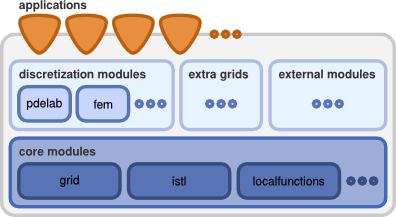
\includegraphics[height=4.2cm]{dunedesign}
		\caption{Tomado de \url{https://dune-project.org}.}
	\end{figure}

\end{frame}

\begin{frame}
	\frametitle{\secname}
	\framesubtitle{\subsecname}

	\begin{columns}
		\begin{column}{0.5\textwidth}
			\begin{alertblock}{Proyectos que emplean DUNE}
				\begin{itemize}
					\item \url{https://dune-project.org/about/dune}
					\item \url{https://dumux.org}
					\item \url{https://opm-project.org}
					\item \url{https://precice.org}
					\item \url{https://www.zib.de/projects/kaskade7-finite-element-toolbox}
				\end{itemize}
			\end{alertblock}
		\end{column}

		\begin{column}{0.5\textwidth}
			\begin{figure}[ht!]
				\centering
				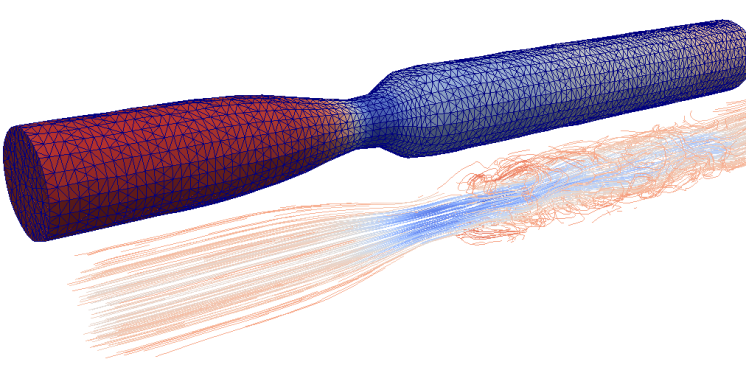
\includegraphics[width=7.5cm]{blood_girke}
				\caption{Tomado de \url{https://dune-project.org}.}
			\end{figure}
		\end{column}
	\end{columns}
	\note{
		Presento las tres primeras páginas, la última versión estable de DUNE es 2.7.1, pero la versión 2.8 se lanzó en septiembre del 2021.

		DuMux es un software basado en modelos, de la química, de los sueles.

		Una característica de OPM es que cuenta con sus propios visualizador de simulación llamado Resinsight.
	}
\end{frame}